%==============================================================
% Springer Requirements Engineering (RE) journal draft
% Compile with XeLaTeX (Chinese body via xeCJK + Fandol fonts)
% Class: svjour3 (Springer journal generic class, bundled in TeX Live/Overleaf)
% For final submission, migrate to the official Springer Nature template (sn-jnl).
%==============================================================
% 说明：Springer 的 svjour3.cls / sn-jnl.cls 均未预装在 Overleaf，
% 故撰写阶段使用 Overleaf 自带、原生支持中文的 ctexart（编译器选 XeLaTeX）。
% 投稿前再迁移到官方 Springer Nature 模板（见 README_OVERLEAF.md）。
\documentclass[a4paper,11pt]{ctexart}

\usepackage{geometry}
\geometry{margin=1in}
\usepackage{graphicx}
\usepackage{amsmath,amssymb}
\usepackage{booktabs}
\usepackage{tabularx}
\usepackage{array}
\usepackage[hidelinks]{hyperref}

\begin{document}

\title{Beyond Majority Vote: Improving Per-Requirement Quality Assessment via Good Outlier Recognition and Roundtable Consensus}

\author{Author One \and Author Two \and Author Three \\[4pt]
\small Affiliation, City, Country \\
\small \texttt{author.one@example.com}}

\date{Received: date / Accepted: date}

\maketitle

\begin{abstract}
在软件工程生命周期中，需求规格说明书的高质量评估对系统成败至关重要。尽管大语言模型（LLM）在自动化需求审查中展现出巨大潜力，但现有的多智能体协作方法普遍陷入“趋同即正确”的共识谬误（Consensus Fallacy）。这种基于多数表决或均值聚合的机制，极易抹杀那些能够揭示深层缺陷、具有极高审查价值的少数派意见（即离群点）。为打破这一局限，本文提出了一种面向逐条需求（per-requirement）质量评估的“离群感知多 LLM 协作工作流”。该框架要求异构模型在四个核心质量维度（可理解性、无歧义性、正确性、可验证性）上独立输出结构化评审；随后引入六维论证质量向量，从文本逻辑层面精准甄别“好离群”与“坏离群”。在此基础上，本研究采用贝叶斯启发式的定权策略，将模型捕捉高价值离群的真实表现转化为静态画像权重，并在条目级多轮圆桌共识中融合该固定权重与模型的动态置信度。我们在真实的公共需求数据集（PURE）上，使用 5 款主流异构 LLM 开展了严密的实证研究。结果表明，多 LLM 在需求质量（尤其是可验证性）判断上存在显著的结构性分歧；所提框架能够有效穿透数值偏差，精准阻断缺乏依据的模型幻觉，同时系统性地放大具备深度逻辑发现能力的少数派洞见。相较于单模型与等权聚合基线，该方法在不追求绝对评分一致的前提下，大幅压缩了冗余候选缺陷，生成了集合高度稳定、精确率更高且具备强工程可操作性的团队级问题清单，为自动化需求质量保证提供了一种打破多数表决范式的全新路径。

\medskip
\noindent\textbf{Keywords:} Requirements quality $\cdot$ Large language models $\cdot$ Multi-agent consensus $\cdot$ Disagreement $\cdot$ Outlier detection $\cdot$ Requirements review
\end{abstract}

\section{Introduction}
\label{sec:introduction}
在现代软件工程生命周期中，软件需求规格说明书（Software Requirements Specification, SRS）的质量直接决定了后续架构设计、编码实现与系统测试的成败。传统的需求质量保证主要依赖领域专家的专家评审或基于规则的静态分析（如需求坏味道 smell 检测），这些方法不仅耗时耗力，且难以深入理解复杂的自然语言语义边界。近年来，随着大语言模型（LLMs）在自然语言处理与推理任务上展现出卓越的能力，研究者开始广泛探索将 LLM 应用于需求工程（RE）领域，以期实现自动化的需求起草、缺陷分类与质量审查。

尽管单一 LLM（LLM-as-a-Judge）在需求质量评估中表现出巨大的潜力，但受限于固有偏置、不可解释的内部逻辑以及偶发的“幻觉”现象，单模型评审在面对复杂工业需求时往往难以提供鲁棒的诊断结论。为此，研究前沿逐渐转向多智能体协作（Multi-Agent Collaboration）与共识机制，期望通过引入多个异构大语言模型进行交叉验证或辩论，以弥补单一模型的认知盲区。然而，现有的多模型集成方法（如多数表决、简单均值聚合，或单纯追求最终输出一致的多轮圆桌讨论）普遍隐式地依赖于一个假设：“趋同即正确”（Consensus Fallacy）。在高度主观且依赖深度逻辑推演的需求质量评审中，这一假设存在致命缺陷。当某个模型的评分严重偏离群体中位数（即触发“离群事件”）时，这并不意味着该模型必然发生了错误。这种偏离既可能是由于幻觉或证据薄弱导致的“坏离群（Bad Outlier）”，也极可能是因为该模型敏锐地捕获了多数模型忽略的隐蔽缺陷，并能提供严密逻辑支撑的“好离群（Good Outlier）”。简单地向多数派或中位数收敛，极易抹杀这些具有极高工程审查价值的少数派洞见。

为了打破多模型需求评审中的“共识谬误”，本文提出了一种面向逐条需求（per-requirement）的“离群感知多 LLM 协作工作流”（Outlier-aware Consensus Workflow）。我们的核心理念是不将多模型间的分歧直接视为需要滤除的随机噪声，而是将其转化为驱动高质量评审的结构化可靠性证据。具体而言，该框架要求异构模型针对需求的可理解性（U）、无歧义性（A）、正确性（C）与可验证性（V）进行独立评分并输出证据与改写建议；随后，框架以中位数为基准自动预筛离群事件，并首创性地引入包含证据充分性、改写可执行性等指标的“六维论证质量向量”，从语义逻辑层面精准甄别好离群与坏离群。在此基础上，本文引入贝叶斯启发式（Bayesian-inspired）的可靠性更新思想：将模型在当前文档中的离群表现累计为模型画像，生成在后续讨论中保持固定的先验权重；最终，在条目级圆桌讨论（Roundtable Consensus）中融合该固定权重与模型的动态置信度，驱动异构模型团队在保留高价值分歧的前提下，收敛至高度结构化的最终问题清单。

为了评估所提框架的有效性与工程实用性，我们在真实的公共需求数据集（PURE）上，利用 5 款主流异构大语言模型展开了严格的组内对照实证研究。通过与单一模型评审、等权聚合基线以及无权重圆桌机制进行严密的消融对比，本文深入探究了异构模型在需求质量评估中的初始分歧结构、论证质量判别的区分效力，以及完整框架在缺陷召回与清单质量之间的性能权衡（Trade-off）。

本文的主要贡献总结如下：
\begin{itemize}
\item \textbf{揭示了多 LLM 需求评审中的结构性分歧规律}：通过实证数据证实了模型在复杂需求缺陷（尤其是“可验证性”与“无歧义性”维度）上极易产生显著的离群判断，证明了将模型分歧视为高价值审查信号的合理性。
\item \textbf{提出并验证了基于论证质量的“好/坏离群”判别与贝叶斯定权机制}：首次在自动化需求评审中实现了从“数值统计聚合”向“文本逻辑验证”的跨越，通过动态提取有效离群证据，有效锚定了各模型在当前评审任务中的真实可靠性。
\item \textbf{构建了融合固定权重与动态置信度的条目级圆桌共识工作流}：实证结果表明，该工作流能够有效抑制低质量偏离，在不追求绝对评分一致的前提下，大幅压缩冗余候选问题，生成集合高度稳定、精确率更高且具备强工程可操作性的团队级缺陷清单。
\end{itemize}

\section{Background and Related Work}
\label{sec:related}
本节我们系统梳理了与本研究相关的三个核心领域，并重点针对该领域的前沿工作与本文的差异进行深度辨论与对比，从而明确本研究在实证软件工程中的学术定位。

\subsection{需求质量评估、需求问题分类与 LLM 在需求工程中的应用}
需求质量评估一直是需求工程中的基础问题，也是软件工程主流研究持续关注的对象[1]。已有研究一方面从系统角度讨论“什么是高质量需求”，指出需求质量研究已经覆盖质量定义、改进技术与评估方法等多个方向[2]；另一方面也强调了该领域长期存在概念碎片化、质量属性界定不统一以及质量评估与后续开发活动之间关联不足的问题[3]。Montgomery 等人的系统映射研究表明，需求质量研究数量已经相当可观，但研究对象、质量属性与评价方式仍然分散[2]；Frattini 等人进一步提出 harmonized theory，强调需求质量研究不能只停留在规范性规则层面，而需要与后续开发活动中的实际影响建立更清晰的联系[3]；Femmer 和 Vogelsang 则从“quality in use”的角度说明，需求质量不应仅被理解为文本是否形式规范，更应关注需求在理解、实现与验证中的实际可用性[4]。对于本文而言，这些工作共同构成了需求质量研究的重要背景，并说明对需求质量的评审必须同时关注文本属性与工程可用性。在更具体的质量问题识别层面，已有研究已经形成了若干具有可操作性的路径。Femmer 等人提出 requirements smells，将模糊、冗余、表述不清等问题视为轻量级质量缺陷，以支持快速质量保证[5]；Lucassen 等人围绕 user story 提出 Quality User Story 框架，将需求质量转化为一组明确可检查的准则[6]；ICSE 社区中的相关工作则进一步从需求质量改进与演化角度，讨论如何通过结构化模式和质量快照分析需求工件的质量状态与变化过程[7][8]。这些研究说明，需求质量并非不可操作的抽象概念，而是可以通过规则、模式或质量指标进行识别和分析。然而，现有工作大多聚焦于单文档规则检查、静态 smell 检测或质量演化分析，通常将自动评估视为单一方法或单一工具的问题，较少讨论多个评审主体在同一 requirement item 上出现显著分歧时应如何处理，更没有将分歧进一步组织为后续权重建模与团队共识的输入。

同时，大语言模型（LLM）在需求工程（RE）中的应用已从简单的文本生成扩展到复杂的质量保证任务。Krishna 等人利用 GPT-4 对 PURE 数据集[9]进行了初步评估，证明 LLM 在起草和审查软件需求规格说明书（SRS）方面具有接近初级工程师的潜力[10]；Zadenoori 等人总结了 LLM 在处理自然语言需求歧义性（Unambiguous）和可测试性（Verifiable）方面的广泛尝试[11]。然而，LLM 在需求审查方面仍存在显著局限，如 Oriol 等人近期发表的 MAD-RE 研究虽然探讨了多智能体辩论（MAD）在需求分类中的应用[12]，但本质上仍将模型视为输出标签的“黑盒”。这类工作侧重于评估模型是否能达成类别一致性，却忽视了需求质量评审的核心——即对分歧语义的深度论证。即模型交互主要集中于达成类别共识，缺乏对“需求歧义点（Evidence）”及“改写策略（Rewrite）”的逻辑链对齐。此外，现有的“LLM-as-a-Judge”范式[13][14]往往面临校准失效的问题。本研究与其不同之处在于，我们不仅要求模型给出 Likert 评分[10]，更通过构建“六维论证质量向量”对模型输出的文本证据进行显式度量，从而弥补现有的 RE-LLM 研究缺乏在 per-requirement 粒度上、基于文本证据深度的冲突调和机制，导致其在处理复杂工业需求时往往陷入“平庸共识”。

\subsection{多 LLM 协作与共识机制}
与单模型 judge 并行发展的是多 LLM 协作、讨论与共识形成研究。该方向的共同假设是：多个模型之间的交流、质疑与说服可以暴露单模型难以发现的推理盲点，并通过多轮互动形成更稳健的集体判断。为了克服单一模型的偏置，学术界提出了多代理对话与写作框架[15--17]。其中，RECONCILE[18]是该领域的里程碑式工作，它提出多轮圆桌会议和置信度加权投票（Confidence-weighted voting）来提升 LLM 的推理一致性。Kaesberg 等人进一步讨论了在不同任务下“Voting”与“Consensus”的优劣[19]。Exchange-of-Thought 则强调 cross-model communication 对复杂问题求解的促进作用[20]；多智能体辩论研究进一步指出，divergent thinking 并非噪声，而可能是提升推理质量的关键资源[16]。整体而言，这些工作共同推动了一个重要转向：在多模型系统中，差异与冲突不一定需要被立即抹平，相反，精心设计的交互过程可能正是产生更优团队决策的前提[16][20]。

对于本文而言，上述研究提供的是机制性基础而非可直接复用的现成方案。现有多 LLM 协作研究大多面向通用推理、问答、数学推导或通用文本评估，较少下沉到需求质量评审这类以工件为中心、以 issue type 为目标输出的任务。同时，这些研究中的讨论对象通常是单一答案或单一判断，而本文的目标是围绕单个 requirement item 在 U/A/C/V 四个维度上形成结构化问题清单，并同时保留 evidence 与 rewrite。再次，已有工作虽然已经区分了 voting 与 consensus 的差异[19]，但在 requirements review 场景中，什么样的决策机制能够既保留多模型分歧的价值、又输出工程上可操作的结果，仍然缺少针对性研究。因此，已有多智能体讨论文献为本文中的“固定权重 + 动态置信度”条目级圆桌共识提供了重要启发，但并没有直接覆盖本文所关注的需求质量审查场景。

\subsection{分歧处理与加权聚合}
在多评审者聚合研究方法论中，如何处理 Disagreement 是一个经典难题。Dawid 和 Skene 的经典工作最早系统讨论了如何从多个观察者的判断中估计其误差率[21]；Whitehill 等进一步研究了未知专长标注者标签的最优整合[22]。Aroyo 和 Welty 提出的“Crowd Truth”理论深刻批判了“唯一正确真理”的迷信，认为分歧往往承载了任务的复杂性[23]。在模型集成领域，Hovy 等人提出的 MACE 模型将标注者能力建模推进到更适合文本任务的聚合框架中，试图通过概率图模型从标注分歧中推断出各标注者的可靠性[24]。这类研究的共同前提是：多个判断来源之间的差异不应被盲目平均，而应显式建模“谁更值得信任”。从这个意义上说，本文根据好/坏离群构造模型画像并进一步生成固定权重，与 reliability-aware weighting 存在明确的方法亲缘性。

但是，传统 reliability-aware aggregation 与本文的方法目标并不相同。经典 annotator aggregation 研究通常假设目标是恢复某种潜在真值，因此 disagreement 往往被视为需要被解释和消解的不确定性来源。与之相比，近年来“learning from disagreement”的研究则指出，在主观性较强或评价标准多元的任务中，分歧本身可能携带有价值的信息，不应一概被压缩成单一标签[25]。同时，针对 instruction-tuned language models 的工作也表明，将多个 LLM 视作“model crowd”是有现实意义的：不同模型确实会在相同任务上呈现系统性标签差异，而聚合方式会显著影响结果质量[26]。本文正是在这一更近的视角上继续推进：我们并不把离群评分直接视为错误，而是进一步追问这些离群中哪些是高价值异议、哪些只是低质量偏离；进一步地，我们也不将权重视为静态先验，而是让权重来源于离群事件的论证质量。正如 Aroyo 等人[23]所指出的，单纯的共识往往是平庸的。我们不从统计概率上惩罚离群（Outliers），而是从语义论证上验证离群。通过六维特征向量，我们能够识别出那些虽偏离中位数、但具备高论证质量的“好离群”。这种从“标签统计”向“文本逻辑验证”的跨越，使得我们能够发现被多数模型忽略的需求缺陷。

\section{Problem Statement and Research Questions}
\label{sec:problem}

\subsection{Problem Statement}
在现代软件工程中，需求规格说明书的高质量评估对整个开发生命周期至关重要。与文档级总体评价不同，本文的分析粒度固定为面向单份需求文档中的逐条需求（per-requirement）质量评估任务，即每条需求都被视为独立的评审单元。给定包含若干需求条目的输入集合，引入多个异构大语言模型（LLMs，记为评估者），针对可理解性（Understandable, U）、无歧义性（Unambiguous, A）、正确性（Correctness, C）、与可验证性（Verifiable, V）四个维度，分别输出基于 Likert 1--5 数量表的评分，以及相应的置信度、证据片段与改写建议。研究的最终输出旨在超越简单的文档级分数聚合，为每条需求提供包含“条目编号、问题类型、证据片段、建议改写及影响力”的团队级诊断结论。

然而，在多 LLM 协作的需求质量评审场景中，不同模型对同一需求条目及同一质量维度的判断往往存在分歧。这种分歧并非偶然的随机噪声，而是由模型底层架构、训练数据、对齐策略、推理风格以及对需求语义边界的不同理解共同导致的结构性现象。传统多数表决或均值聚合机制通常隐含一个前提：越接近群体中心的判断越可靠，越偏离共识的判断越可疑。但在需求质量评审中，这一假设并不充分成立。某个模型给出的偏离评分既可能源于幻觉、误解或弱证据推断，也可能意味着该模型捕获了其他模型忽略的隐蔽缺陷。因此，“离群”本身并不必然等同于错误；关键问题在于如何判断一个偏离判断是否具有审查价值。

具体而言，对于任意需求条目与质量维度，本文以所有模型评分的中位数作为群体基准。当某一模型评分满足离群条件时，该评分被识别为一个“离群”事件。此时该离群事件可能属于两种性质完全不同的情形：一种是“坏离群（Bad Outlier）”，即评分显著偏离群体基准，但缺乏充分证据、存在维度错配或无法给出可执行改写；另一种是“好离群（Good Outlier）”，即评分虽然偏离多数模型判断，但能够提供明确证据、合理解释和可操作的修改建议，从而揭示被多数模型忽略的潜在需求缺陷。若直接采用多数表决或向中位数收敛的策略，前者可能被错误保留，后者则可能被过早抹平。

因此，本文要解决的核心问题不是“如何让多模型评分更接近一致”，而是“如何识别哪些分歧具有审查价值，并将这种价值稳定地转化为最终团队结论”。这一问题包含三个连续挑战。首先，需要在 per-requirement 粒度下刻画多异构 LLM 初始评分的分歧结构，识别哪些需求条目与质量维度更容易触发强离群事件。其次，需要进一步判断离群事件的质量，即区分具有充分证据和可执行改写的高价值离群意见，以及由幻觉、弱证据或维度误判导致的低质量偏离。最后，需要将离群质量判别结果转化为模型级可靠性估计，并在条目级圆桌共识中与模型的动态置信度结合，生成更稳定、更聚焦且更具工程可用性的团队级问题清单。

从不确定性建模角度看，多 LLM 需求质量评审可以被理解为一个多观察者推断问题。对于任意需求条目及其质量维度，真实缺陷状态并不能被模型直接观测，而只能通过多个模型给出的评分、置信度、证据片段和改写建议间接反映。换言之，每个模型输出都不是确定性真值，而是带有模型偏好、推理能力差异与潜在幻觉风险的“noisy observation”。在这一视角下，多模型聚合的关键不只是对多个评分求平均，而是在缺乏直接真值的条件下，根据模型在当前文档中的输出质量与离群表现，更新对其审查可靠性的估计，并进一步推断某一候选缺陷是否应被保留为团队级结论。

基于这一认识，本文将好离群与坏离群视为模型可靠性更新的观测证据。若某模型多次产生偏离中位数但证据充分、维度匹配且改写可执行的判断，则这些事件应构成提升其后续影响力的正向证据；相反，若某模型频繁产生证据缺失、维度错配或改写不可落地的偏离判断，则这些事件应构成削弱其后续影响力的负向证据。因此，本文不预设所有模型在需求评审任务中具有相同可靠性，也不依据通用 benchmark 或模型推理能力进行静态排序，而是依据当前需求文档中的好/坏离群表现构建任务内、文档内的模型画像。进一步地，本文采用带有保守先验约束的贝叶斯式可靠性更新思想，将好离群强度与坏离群强度分别视为支持或削弱模型可靠性的证据，并据此形成后续圆桌共识阶段使用的固定模型权重。

这一设定使本文区别于三类常见方法。第一，本文不同于单模型需求评审，因为它不依赖某一模型独立完成缺陷判断，而是利用异构模型之间的差异作为信息来源。第二，本文不同于简单等权聚合，因为它并不假设所有模型输出具有相同可信度，而是根据模型在当前文档中的离群质量表现调整其后续影响力。第三，本文也不同于单纯追求一致性的多智能体讨论，因为它并不将分歧本身视为需要消除的噪声，而是将分歧进一步拆解为高价值异议与低质量偏离，并利用这种区分结果驱动模型定权与团队共识生成。

综上，本文研究的问题可以概括为：在面向逐条需求的 U/A/C/V 质量评估任务中，如何将多 LLM 的结构化分歧从简单的评分偏差转化为可解释的可靠性证据，并进一步利用这种证据驱动模型权重更新与条目级圆桌共识形成。为此，本文构建一条从初始评分分歧识别、离群事件质量判别、模型画像与后验式权重构造，到固定权重与动态置信度融合的团队级问题清单生成的完整决策链。该框架旨在避免“趋同即正确”的共识谬误，在抑制低质量偏离的同时保留并放大具有工程审查价值的少数派意见。

\subsection{Research Questions}
基于上述问题陈述，本文提出以下三个研究问题。三个研究问题分别对应本文研究逻辑中的三个层次：首先分析单个 LLM 在逐条需求质量问题识别中的差异性；其次评估本文提出的离群感知共识流程相对于单模型和传统聚合基线的表现与权衡；最后进一步考察该方法在不同需求文档和质量维度下的表现变化。

\begin{description}
\item[RQ1.] How do individual LLMs differ in identifying per-requirement quality issues in software requirements? \\
RQ1 关注单个 LLM 在逐条需求质量问题识别中的差异性。具体而言，本文分析不同 LLM 在 U/A/C/V 四个质量维度上的评分分布、证据使用、问题类型识别、维度敏感性以及离群行为是否存在系统差异。该问题的目的在于刻画多模型初始判断之间是否存在可观察、可分析的结构性分歧，从而为后续引入多 LLM 协同机制和离群感知处理提供经验基础。
\item[RQ2.] How does the proposed outlier-aware consensus workflow compare with individual LLMs and aggregation baselines in producing per-requirement quality issue lists? \\
RQ2 关注本文提出的离群感知共识流程在生成逐条需求质量问题清单时，相较于单模型评审和传统聚合基线表现出怎样的效果与权衡。该问题并不预设本文方法必然在所有指标上优于基线，而是考察其在 Ground Truth 对齐、问题清单规模、证据支持、集合收敛性和人工审查可用性等方面的综合表现。
\item[RQ3.] How does the performance of the consensus workflow vary across requirements documents and quality dimensions? \\
RQ3 关注本文提出的共识流程在不同需求文档和不同质量维度下的表现差异。该问题旨在识别共识流程在哪些文档或质量问题类型上更有效，以及在哪些场景下仍然存在局限，从而揭示本文方法的适用边界。
\end{description}

\section{Methodology}
\label{sec:method}
本研究构建了一种融合多大语言模型与动态圆桌共识机制的自动化需求质量评估框架，其核心目标是在单份需求文档内部，以 per-requirement 为分析粒度，将多个异构大语言模型对同一需求条目的质量判断、证据与改写建议组织为可解释、可复现的团队级问题清单。设待评估的需求条目集合为 $\mathcal{I}=\{1,\dots,n\}$，评价维度集合限定为 $\mathcal{D}=\{U,A,C,V\}$，分别对应可理解性 Understandable、无歧义性 Unambiguous、正确性 Correctness 与可验证性 Verifiable。

对于任意模型或评分者 $r\in\mathcal{R}$、需求条目 $i\in\mathcal{I}$ 以及维度 $d\in\mathcal{D}$，模型输出一个 Likert $1..5$ 的评分 $s_{r,i,d}$，并提供相应的置信度、证据片段与建议改写。本文的方法流程通过以下七个阶段，将多模型的异质化评分转化为可复现的团队级需求诊断清单：多 LLM 逐条需求结构化评分、基于中位数的离群事件自动预筛、论证质量向量评分、好离群/坏离群判别、模型画像与权重构造、固定权重与动态置信度融合的条目级圆桌共识，以及最终问题清单提取。

为增强模型定权过程的统计解释性，本文进一步从贝叶斯可靠性更新的视角解释多 LLM 协同评审过程。模型在当前文档中产生的好离群与坏离群，分别被视为支持或削弱其可靠性的观测证据。基于这一设定，本文的模型定权过程可以被理解为：先对每个模型赋予均匀且保守的先验信任，再根据当前文档中好/坏离群的观测结果更新其后验可靠性，并将该后验可靠性转化为后续圆桌共识阶段的固定模型权重。这种贝叶斯式解释并不改变本文原有的离群定义、论证质量向量或圆桌共识流程，而是为“为什么好离群应当升权、坏离群应当降权”提供更明确的概率化依据。

\begin{figure}[t]
\centering
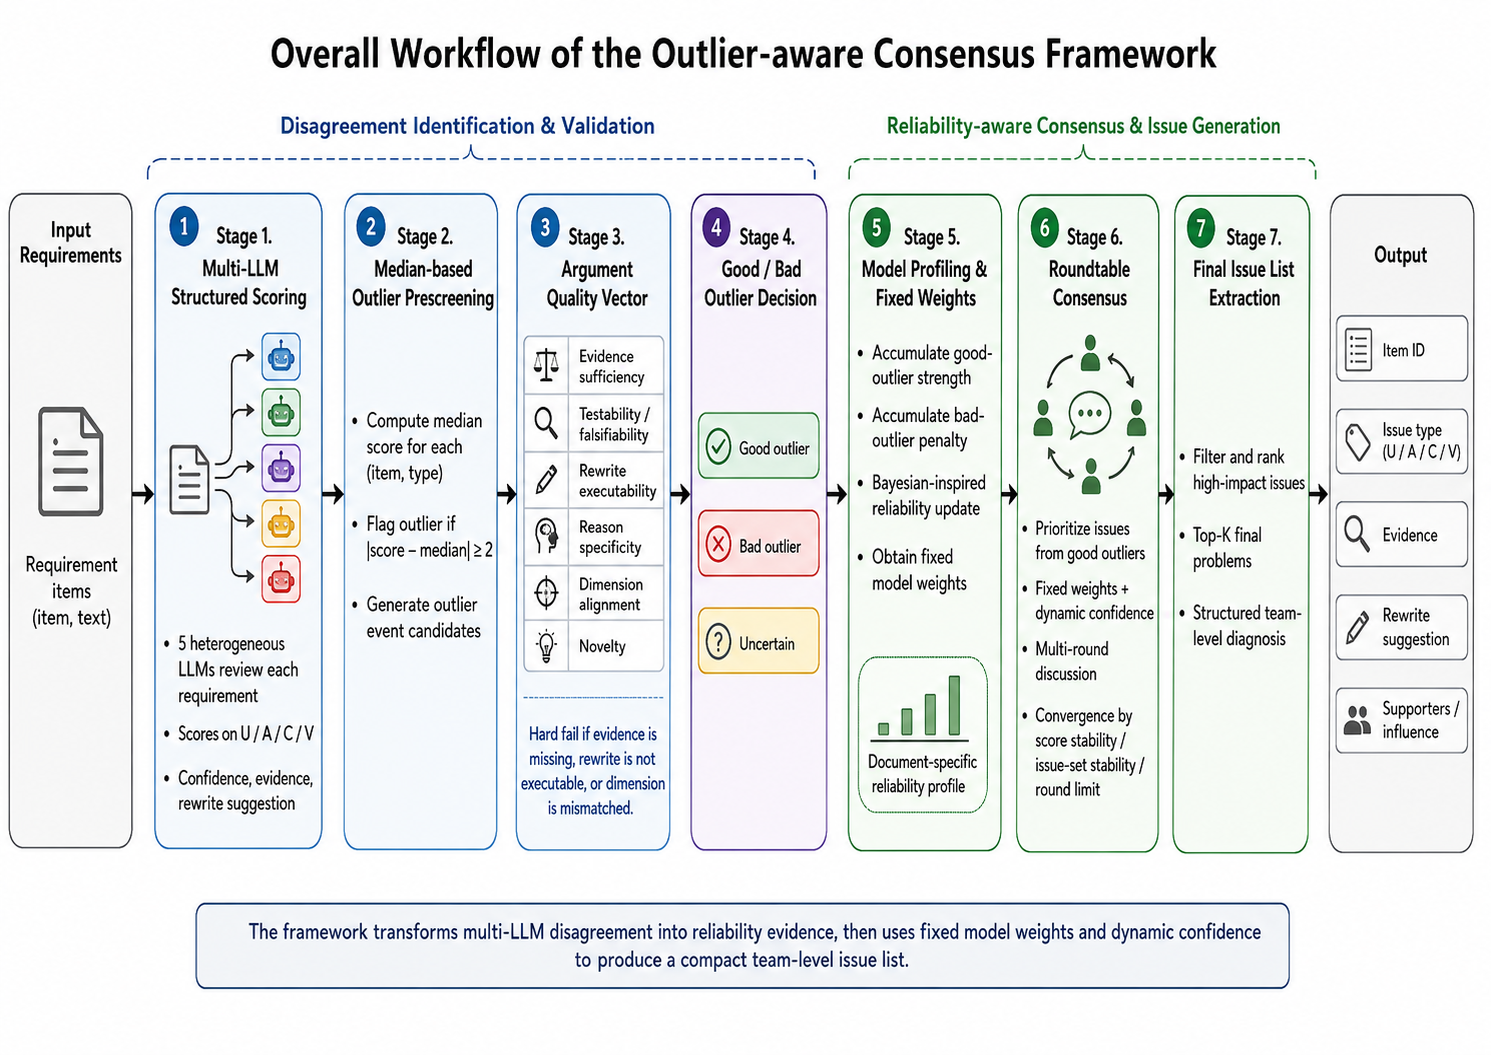
\includegraphics[width=\linewidth]{figures/fig1_overall_workflow.png}
\caption{Overall workflow of the proposed outlier-aware multi-LLM consensus framework.}
\label{fig:overall_workflow}
\end{figure}

\subsection{阶段 1：多 LLM 逐条需求结构化评分}
在该阶段，鉴于分析粒度严格限定为逐条需求（per-requirement），我们输入包含需求编号（item）与需求原文（text）的需求条目表 requirements，同时引入多个异构 LLM（记为评估者）作为虚拟评审员。对每条需求，系统调用每个模型针对需求条目在维度上进行独立推断，依据 $1..5$ 分的 Likert 量表对单条需求独立评分。每个模型必须输出四维评分、初始置信度、相对应的原文证据片段（evidence），以及原子化、无歧义且可执行的建议改写（rewrite\_suggestion）。该阶段承担两个基础功能：其一，它将多模型意见统一到相同维度协议和相同数值区间内，使后续的离群识别具有可比较性；其二，它显式地保留证据与改写建议，而不是仅保留数值评分，从而为后续论证质量判定和圆桌讨论提供可审查的语义材料。

\subsection{阶段 2：离群事件自动预筛}
多 LLM 评分往往存在显著分歧。本阶段旨在从海量评分长表中识别出严重偏离群体共识的“离群事件”（Outlier Events），以作为后续深度审查的重点。针对阶段 1 产出的全量结构化结果集合，为消除单一模型偏差，我们以模型群体的中位数作为一致性基准。对于每个需求条目和每个维度，我们首先以所有评分者在该二元组上的评分集合构造中位数基准：
\begin{equation}
% TODO: 原 main.docx 中位数基准公式，提取时丢失，请从 docx 公式对象复制
\tilde{s}_{i,d} = \operatorname{median}\{\, s_{r,i,d} : r \in \mathcal{R} \,\}.
\end{equation}
并在此基础上，对每个评分计算偏差与绝对偏差：
\begin{equation}
\delta_{r,i,d} = s_{r,i,d} - \tilde{s}_{i,d}, \qquad |\delta_{r,i,d}|.
\end{equation}
设定离群敏感阈值 $\theta=2$ 执行自动预筛。因此，当 $|\delta_{r,i,d}| \ge \theta$ 时，判定该三元组触发离群事件。相应的输出为离群事件集合，作为后续论证质量评估的候选池。需要指出的是，本阶段的目的不是将偏离共识的判断直接视为错误，而是构建一个“需要重点审查”的候选集合。

\subsection{阶段 3：论证质量向量评分}
离群并不必然代表错误（“坏离群”），它也可能是模型发现了隐蔽缺陷并给出了高质量论证（“好离群”）。本阶段旨在通过六维特征对离群事件的文本输出进行深度质量量化。每个离群事件都要被映射为一个六维论证质量向量，六个子项分别为：证据充分性、可证伪/可测试性、改写可执行性、理由具体性、维度匹配度与新颖性。其归一化论证质量分 $Q$ 定义为：
\begin{equation}
% TODO: 原 main.docx 论证质量归一化分 Q 的公式，提取时丢失，请从 docx 复制
Q = \text{[公式待补：六维子项的均匀归一化]}.
\end{equation}
同时，我们设定严格的“硬性否决”（Hard Fail）机制：若证据充分性、改写可执行性或维度匹配度任一子项为 $0$，则该离群事件直接被判定为“坏离群”。

\subsection{阶段 4：好/坏离群判别}
本阶段建立自动化判别逻辑，对离群事件的性质进行分类定性。在不改变离群定义的前提下，对每个已识别离群事件设定经验判定阈值作为自动判别边界：若 $Q \le \tau_{bad}$，则判定为坏离群（bad）；若 $Q \ge \tau_{good}$，则判定为好离群（good）；介于二者之间的灰色地带离群定义为不确定事件（Uncertain），用于后续仅在必要时通过“自动预筛 + 少量人工确认”覆写。其中 $\tau_{good}=0.60$，$\tau_{bad}=0.30$。由此可得到包含离群标签的判别表，为后续模型权重学习提供监督信号。这一判别机制体现了本文与简单的“偏差越大越可疑”策略的根本区别：离群信息从“异常值”被重新定义为“具有不同审查价值的异议样本”。

\subsection{阶段 5：模型画像与权重构造}
区别于传统集成学习中平权的投票机制，本框架依据各模型处理离群事件的能力对其分配不同的全局固定权重。该权重并不表示模型在所有任务上的通用能力排序，而是表示模型在当前文档、当前需求质量评审任务下，由好/坏离群证据诱导出的相对审查可靠性。本阶段将离群事件级别的质量判断累积为模型级画像，并据此构造在后续圆桌中保持固定的模型权重。对任意模型，我们定义其正向贡献（好离群强度 $G_r$）与负向惩罚（坏离群强度 $B_r$）：
\begin{equation}
% TODO: 原 main.docx 中 G_r 与 B_r 的累计定义公式，提取时丢失，请从 docx 复制
G_r = \text{[公式待补]}, \qquad B_r = \text{[公式待补]}.
\end{equation}
为了避免 1$\sim$2 个好/坏离群在小样本场景下直接主导后续圆桌，我们先计算引入平滑常数 $\kappa$ 的当前文档证据分数：
\begin{equation}
\mathrm{score}_{doc}(r) = \frac{G_r - \lambda B_r}{\kappa + n_{good}(r) + n_{bad}(r)}.
\end{equation}
其中，$\kappa>0$ 为分母平滑项，可理解为一个保守的先验样本量项。本文将 $\kappa$ 固定设为 $3.0$，使得在当前文档仅出现 1 至 2 个有效好/坏离群时，模型权重仅发生温和调整，而不被单个离群事件主导。考虑到本文未引入独立的跨文档校准集，在观察当前文档中的有效离群证据之前，我们对所有参与模型赋予相同的先验信任度。记当前文档的有效离群证据总量与文档证据强度为：
\begin{equation}
% TODO: 原 main.docx 中有效离群证据总量与文档证据强度公式，提取时丢失
n_{eff} = \text{[公式待补]}, \qquad \text{evidence strength} = \text{[公式待补]}.
\end{equation}
其中文档级先验强度 $\eta$ 用于控制当前文档证据相对于默认先验的更新幅度，本文将其固定设为 $4.0$。当前文档诱导的 Softmax 权重以及最终用于条目级圆桌的固定权重为：
\begin{equation}
% TODO: 原 main.docx 中 Softmax 权重与最终固定权重公式，提取时丢失
w_r = \operatorname{softmax}\big(\eta \cdot \mathrm{score}_{doc}(r)\big), \qquad w_r^{\,*} = \text{[公式待补：归一化]}.
\end{equation}
该固定权重并不作为独立的最终输出，而是作为后续条目级圆桌共识中的先验影响力项，其实际贡献将在完整方法与无权重圆桌的消融比较中进行评估。

\subsection{阶段 6：融合固定权重与动态置信度的条目级圆桌共识}
为模拟真实的评审会议，我们受 RECONCILE 框架启发，本阶段在单条需求内部开展多轮意见交互。圆桌遵循三个不可更改的核心约束：第一，圆桌中不显式讨论“离群”概念，离群仅用于事前权重分配；第二，模型权重在整个圆桌过程中固定不变；第三，代表模型当前确信度的置信度随模型间的多轮交互动态更新。在候选问题构造上，我们优先使用好离群对应的二元组作为候选问题集合，以确保好离群优先在圆桌中讨论；当该集合不足以支撑讨论时，允许回退到全量问题集合。对任意模型、需求条目与维度，定义其在该问题上的影响力，并将支持该问题的模型集合进行影响力聚合，得出该问题的团队得分：
\begin{equation}
% TODO: 原 main.docx 中影响力与团队得分公式，提取时丢失，请从 docx 复制
\mathrm{infl}_{r,i,d} = \text{[公式待补]}, \qquad S_{i,d} = \sum_{r \in \mathrm{Supp}(i,d)} \mathrm{infl}_{r,i,d}.
\end{equation}
在每轮按团队得分对候选问题进行排序，并以排序结果组织后续讨论。圆桌的终止条件同时保留三类：分数收敛、问题集合收敛（以集合重叠度刻画）以及固定轮次上限。

\subsection{阶段 7：最终问题清单提取}
最后阶段依据共识机制的量化结果提取可供软件工程团队直接使用的优化建议。针对圆桌共识结束后得到的团队问题得分、对应证据片段以及改写建议，我们引入筛选置信阈值进行筛选，提取最终高质量问题集合：
\begin{equation}
% TODO: 原 main.docx 中最终问题集合提取阈值公式，提取时丢失，请从 docx 复制
\text{final issues} = \{(i,d) : S_{i,d} \ge \text{threshold}\}.
\end{equation}
符合条件的问题将按降序排列，筛选出 Top-K（例如 10 项）最具高影响力的缺陷条目，并最终形成高度结构化的团队级结论，其标准化输出为：条目编号 + 问题类型（U/A/C/V）+ 证据片段 + 建议改写（+ 支持者/影响力）。

\section{Experimental Design}
\label{sec:experiment}
本章旨在阐述评估本文提出的多 LLM 协同需求质量审查框架的实证研究设计。结合前述的三个研究问题（RQs），实验设计遵循一条由浅入深的验证逻辑：首先刻画多异构 LLM 在初始评分阶段的分歧特征（RQ1）；其次通过严格的控制变量与消融基线，评估本文提出的完整共识工作流在问题清单生成上的综合表现及其内部机制（RQ2）；最后进一步探究该方法在不同需求文档特征与不同质量维度下的泛化能力与表现差异（RQ3）。

\subsection{实验目标与分析单元（Experimental Objectives and Evaluation Unit）}
本文的实验单位严格固定为单份需求文档内部的 per-requirement 评估。对于每条需求，系统分别在可理解性（U）、无歧义性（A）、正确性（C）与可验证性（V）四个维度上进行判断。因此，本实验的最小评价单元被定义为二元组 $(item,type)$，其中 item 表示需求条目编号，$type\in\{U,A,C,V\}$。本实验不仅评估模型的数值评分表现，更关注最终能否生成包含证据片段和建议改写的结构化团队级诊断结论。

\subsection{实验对象与数据集（Subjects and Datasets）}
\subsubsection{评估对象（异构 LLMs）}
本实验选取了 5 款当前主流且底层架构存在差异的大语言模型作为虚拟评审员，分别为 DeepSeek-Reasoner、Qwen-plus、GPT-5.1、Kimi-k2-0905-preview 和 GLM-5。这种异构设计旨在最大程度地真实模拟专家评审团队中由于背景知识、训练语料和推理偏好不同而产生的视角差异，从而为“分歧处理”提供充足的实验载体。

\subsubsection{实验数据集（Datasets）}
\label{sec:datasets}
实验采用广泛用于实证软件工程研究的公共需求文档数据集 PURE（PUblic REquirements dataset）。该数据集包含来自真实工业界和开源项目的软件需求规格说明书（SRS）。实验采用分层抽样，筛选了 10 份覆盖不同业务领域、不同规模（从数十条到数百条需求不等）的文档，以确保结论不依赖于单一上下文。该子集共包含 978 条需求条目与 3,912 个 $(item,type)$ 评价单元。PURE 数据集保留了自然语言需求中真实存在的模糊、冗余和逻辑不一致等缺陷，且支持被解析为统一的 $(item, text)$ 结构，完美契合本研究的细粒度分析需求。

\input{tables/table_01.tex}

\subsection{实验处理与基线设置（Treatments and Baselines）}
\label{sec:treatments}
为准确回答 RQ2，隔离并量化本文方法中各模块的实际贡献，同一份需求文档将在以下四种处理条件（Treatments）下进行并行评估：
\begin{itemize}
\item \textbf{Single-LLM（单一模型）}：由 5 个 LLM 分别独立完成四维评分与问题输出，作为各模型在当前任务上的基础表现下界。
\item \textbf{Equal-Weight Aggregation（等权聚合）}：多模型独立评分后，不引入论证质量判别与离群定权，直接按照等权重原则进行 issue 分数聚合，用于评估“单纯增加模型数量”带来的基线提升。
\item \textbf{Roundtable No Weighting（无权重圆桌）}：保留多轮动态置信度与圆桌讨论机制，但剥离贝叶斯更新权重，使所有模型在讨论中保持等权参与。
\item \textbf{Full Method（完整方法）}：采用本文构建的“结构化评分 $\to$ 离群质量判别 $\to$ 证据驱动型后验定权 $\to$ 动态置信度圆桌共识”的完整决策链。
\end{itemize}
特别地，实验设计了严密的消融对比逻辑：通过比较 Full Method 与 Roundtable No Weighting，隔离“证据驱动型固定模型权重”的贡献；通过比较 Roundtable No Weighting 与 Equal-Weight Aggregation，分析“多轮圆桌讨论机制”本身的贡献；通过比较 Full Method 与 Single-LLM，评估完整框架相较单模型评审的总体增益。

\begin{table*}[t]
\centering
\caption{Treatments, baselines, and ablation settings.}
\label{tab:treatments_baselines}
\renewcommand{\arraystretch}{1.15}
\resizebox{\textwidth}{!}{%
\begin{tabular}{p{2.6cm}p{3.2cm}p{2.2cm}p{2.2cm}p{2.2cm}p{4.0cm}}
\toprule
\textbf{Treatment} &
\textbf{Input and aggregation setting} &
\textbf{Outlier quality validation} &
\textbf{Fixed model weights} &
\textbf{Roundtable discussion} &
\textbf{Purpose in evaluation} \\
\midrule

\textbf{Single-LLM} &
Each LLM independently produces U/A/C/V scores, confidence, evidence, and rewrite suggestions for each requirement. No cross-model aggregation is applied. &
No &
No &
No &
Estimates the standalone capability of individual LLM reviewers and serves as the lower-level reference for assessing the benefit of multi-LLM collaboration. \\

\midrule

\textbf{Equal-Weight Aggregation} &
All LLMs share the same round-0 structured outputs. Candidate issue scores are aggregated under equal model influence. &
No &
No; all models are treated equally. &
No &
Tests whether simply combining multiple LLMs improves issue-list generation without disagreement validation or interactive consensus. \\

\midrule

\textbf{Roundtable No Weighting} &
Uses the same round-0 outputs and candidate issues as the other multi-LLM settings. Models participate in multi-round discussion. &
No explicit good/bad outlier validation for model weighting. &
No; all models retain equal influence during discussion. &
Yes; dynamic confidence is updated across rounds. &
Isolates the contribution of the roundtable discussion mechanism while removing reliability-aware fixed weights. \\

\midrule

\textbf{Full Method} &
Uses the complete structured scoring output, including scores, confidence, evidence, and rewrite suggestions. &
Yes; outlier events are assessed using the argument quality vector and hard-fail rules. &
Yes; document-specific fixed weights are derived from good- and bad-outlier evidence. &
Yes; fixed weights are combined with dynamic confidence during multi-round consensus. &
Evaluates the complete outlier-aware consensus workflow, including disagreement validation, model profiling, and roundtable-based final issue-list extraction. \\

\bottomrule
\end{tabular}%
}

\vspace{0.4em}
\begin{minipage}{0.97\textwidth}
\footnotesize
\textit{Note.} All treatments are evaluated on the same requirement documents and share the same initial round-0 LLM outputs whenever applicable. This paired design controls for stochastic variation in LLM generation and allows the ablation comparisons to isolate the effects of equal aggregation, roundtable discussion, and reliability-aware fixed weighting.
\end{minipage}
\end{table*}


\subsection{度量指标与 Ground Truth 构建（Metrics and Ground Truth）}
\label{sec:metrics}
为评估最终生成的缺陷清单质量，本研究采用专家交叉盲标的方式构建 Ground Truth（GT）。邀请两名具备数年需求工程经验的专家，对所有 $(item, type)$ 二元组独立标注是否存在对应缺陷；针对分歧项，由第三名资深专家引入讨论并仲裁。专家间的初始一致性通过 Cohen's Kappa 或 Krippendorff's $\alpha$ 予以严谨报告。针对三个 RQ，定义如下量化指标：RQ1（初始评分分歧）使用序数型 Krippendorff's $\alpha$ 度量模型初始评分的一致性，并统计判定为离群的事件频率及其在各维度的分布；RQ2（论证质量判别）计算论证质量归一化分 $Q$，统计因证据缺失、维度错配或改写不可执行而触发“硬性否决（Hard Fail Rate）”的离群事件占比；RQ3（团队清单质量与收敛性）鉴于四类缺陷在真实文档中分布极度不均衡，选用 Macro-F1 作为核心性能主指标，同时报告 Macro-Precision、Macro-Recall，以及相邻圆桌轮次间候选缺陷集合的 Jaccard 相似度。

\subsection{控制变量与复现控制（Control Variables and Reproducibility）}
为最大限度降低内部效度威胁，本实验实施了严格的复现控制：（1）\textbf{共享初始状态}：所有聚合方法与圆桌基线共享同一批 round-0 模型输出（初始评分、置信度、证据片段），彻底排除 LLM API 采样随机性导致的不同方法间输入不一致问题；（2）\textbf{统一参数配置}：所有文档共享固定的超参数：离群阈值 $\theta=2$；好/坏离群阈值 $\tau_{good}=0.60$、$\tau_{bad}=0.30$；贝叶斯平滑项 $\kappa=3.0$、$\eta=4.0$；Softmax 惩罚系数 $\lambda=1.5$；圆桌讨论最大轮次 $\mathrm{rounds}=2$；（3）\textbf{系统稳健性控制}：系统部署了指数退避重试机制，若某模型在特定需求条目上历经最大重试依然失败，系统将在当前 case 中执行单模型隔离（跳过该模型），其余模型继续执行共识机制，从而真实验证本框架在“评审成员缺席”环境下的鲁棒性。

\subsection{数据分析与统计方法（Data Analysis Methods）}
\label{sec:analysis}
统计分析严格以“Document”为单位进行 Block 处理，以防止直接混合异质需求条目引发辛普森悖论。本文统一采用 $\alpha=0.05$ 作为显著性水平，并同时报告非参数效应量，结合显著性与实际指标提升幅度共同解释实验结果。解答 RQ1（分歧结构）采用 Friedman 检验分析不同质量维度（U/A/C/V）触发强离群事件的频率是否存在显著差异；解答 RQ2（判别有效性）采用 Mann--Whitney U 检验比较“好离群”与“坏离群”在 $Q$ 分数及子维度得分上是否实现显著分离，并计算 Cliff's $\delta$ 效应量；解答 RQ3（框架性能与消融）由于同一份文档在四种处理条件下均被评估，采用全局 Friedman 检验分析 Macro-F1 等指标的差异，若全局差异显著则使用 Holm--Bonferroni 事后校正依次进行两两成对比较，同时绘制 Jaccard 相似度曲线与分数波动衰减图，直观展示系统的收敛轨迹。

\begin{table*}[t]
\centering
\caption{Evaluation metrics and statistical tests by research question.}
\label{tab:metrics_tests_by_rq}
\renewcommand{\arraystretch}{1.15}
\resizebox{\textwidth}{!}{%
\begin{tabular}{p{1.1cm}p{3.1cm}p{4.1cm}p{3.7cm}p{3.0cm}}
\toprule
\textbf{RQ} &
\textbf{Analysis focus} &
\textbf{Evaluation metrics} &
\textbf{Statistical tests} &
\textbf{Interpretation target} \\
\midrule

\textbf{RQ1} &
Initial differences among individual LLMs in per-requirement quality issue identification. &
Score distribution by dimension; dimension-wise mean and median scores; inter-model agreement using ordinal Krippendorff's $\alpha$; outlier-event count and outlier rate under $|score-median|\geq 2$; distribution of outliers across U/A/C/V. &
Descriptive agreement analysis; Friedman test on document-level outlier rates across U/A/C/V; post-hoc paired Wilcoxon signed-rank tests with Holm correction when needed; non-parametric effect size reporting. &
Determines whether LLM disagreement is random noise or a structured signal that varies systematically by quality dimension. \\

\midrule

\textbf{RQ2} &
Effectiveness and trade-off of the proposed outlier-aware consensus workflow compared with individual LLMs and aggregation baselines. &
Argument quality score $Q$; good/bad/uncertain outlier counts; hard-fail rate; Macro-Precision, Macro-Recall, and Macro-F1 against GT; average predicted issue-list size; issue-set Jaccard similarity; final max score difference; retention and reduction of candidate issues. &
Mann--Whitney U tests for good vs. bad and good vs. non-good outlier separation; Friedman test for document-level comparison across treatments; paired Wilcoxon signed-rank tests with Holm correction for post-hoc treatment comparisons; Cliff's $\delta$ for non-parametric effect size. &
Assesses whether the workflow separates high-value disagreement from low-quality deviation and whether it produces a more compact, stable, and GT-aligned issue list than the baselines. \\

\midrule

\textbf{RQ3} &
Variation of workflow performance across requirements documents and quality dimensions. &
Document-level Macro-Precision, Macro-Recall, and Macro-F1; per-document issue-list size; dimension-wise precision, recall, F1, and final issue distribution; initial-to-final dimension shift; candidate-retention rate by document and by dimension. &
Block-wise descriptive analysis by document; Friedman or Kruskal--Wallis tests for cross-dimension variation when applicable; paired Wilcoxon tests for initial-to-final shifts; Spearman correlation for associations between document characteristics and performance indicators. &
Identifies the contexts and quality dimensions where the workflow is most effective, and clarifies its limits under sparse positives, low defect density, or dimension-specific imbalance. \\

\bottomrule
\end{tabular}%
}

\vspace{0.4em}
\begin{minipage}{0.97\textwidth}
\footnotesize
\textit{Note.} Statistical comparisons are conducted at the document level whenever treatment-level performance is compared, so that each requirements document acts as a paired block. This design avoids treating heterogeneous requirement items as independent observations and reduces the risk of inflated significance caused by document-level heterogeneity.
\end{minipage}
\end{table*}


\section{Results}
\label{sec:results}
本章报告本文三个研究问题的实证结果。所有结果均基于 Ground Truth（GT）、当前多模型输出和文档级统计分析。为保证 Full Method 诊断结果与配对比较（Treatment-level）使用相同的覆盖范围，本章采用 10 份共同需求文档作为统一分析口径。

\subsection{RQ1：How do individual LLMs differ in identifying per-requirement quality issues?}
为刻画 RQ1 所关注的单个 LLM 在逐条需求质量问题识别中的初始判断差异，我们首先对 round-0 评分矩阵（固定所有文档、所有模型采用同一版 prompt、同一版解析脚本、同一组阈值参数，从而保证不同 treatment 的实验起点相同）计算了序数型 Krippendorff's $\alpha$ 指标。结果显示，跨全部 10 份文档、978 条 requirement 与 3{,}912 个 $(item,type)$ 单元的总体一致性为 $0.4232$，说明不同模型在初始评分阶段存在一定程度但不充分的收敛。进一步按维度分解后，U/A/C/V 四个维度的 $\alpha$ 分别为 $0.0258$、$-0.0377$、$0.1202$ 与 $0.0526$，这表明当分析粒度下沉到 U/A/C/V 的细粒度判别任务时，模型间判断没有形成稳定一致性，部分维度甚至表现出低于随机一致性的趋势。

从评分分布看，四个维度的初始评分同样显示出显著的维度间差异。U 与 C 的中位数均为 $3$，A 与 V 的中位数为 $2$；四个维度的平均评分分别为 U$=2.6279$、A$=2.0602$、C$=2.8605$ 和 V$=1.7030$，其中 V 的平均分最低，而 C 的平均分最高。这一结果说明，当前模型群体在可验证性相关判断的初始阶段更容易触发“存在问题”的低分信号，而正确性判断整体上更趋于保守。

在离群预筛阶段（$|score-median|\geq 2$），数据分布显示评分分歧并非随机噪声，而是表现出显著的维度聚集性。我们在 10 份文档中共识别出 60 个 outlier events。按维度统计，V 维度共触发 42 个 outlier，占全部离群事件的 $70.00\%$；U、A 与 C 分别仅有 7 个（$11.67\%$）、6 个（$10.00\%$）与 5 个（$8.33\%$）。若进一步以“文档内离群率”进行归一化，四个维度之间的差异依然显著：V 维度的平均离群率依然最高（$1.26\%$），显著高于 U（$0.20\%$）、A（$0.15\%$）与 C（$0.15\%$）；Kruskal--Wallis 检验验证了这四个维度的文档内离群率存在统计学显著差异（% TODO: 从 main.docx 补全精确统计量，例如 $H$, df, $p$
$p<0.05$）。

\textit{Result for RQ1:} 个体 LLM 在逐条需求质量问题识别中并非仅产生无结构的随机噪声，而是在评分水平、维度敏感性和强分歧触发位置上呈现出可观察的结构性差异。尤其是 V 维度，在当前实验设置下既表现出更低的平均评分，也集中产生最多离群事件。这一结果为本文将“模型分歧”视为可利用的结构化信号提供了坚实的经验基础。

\begin{figure}[t]
\centering
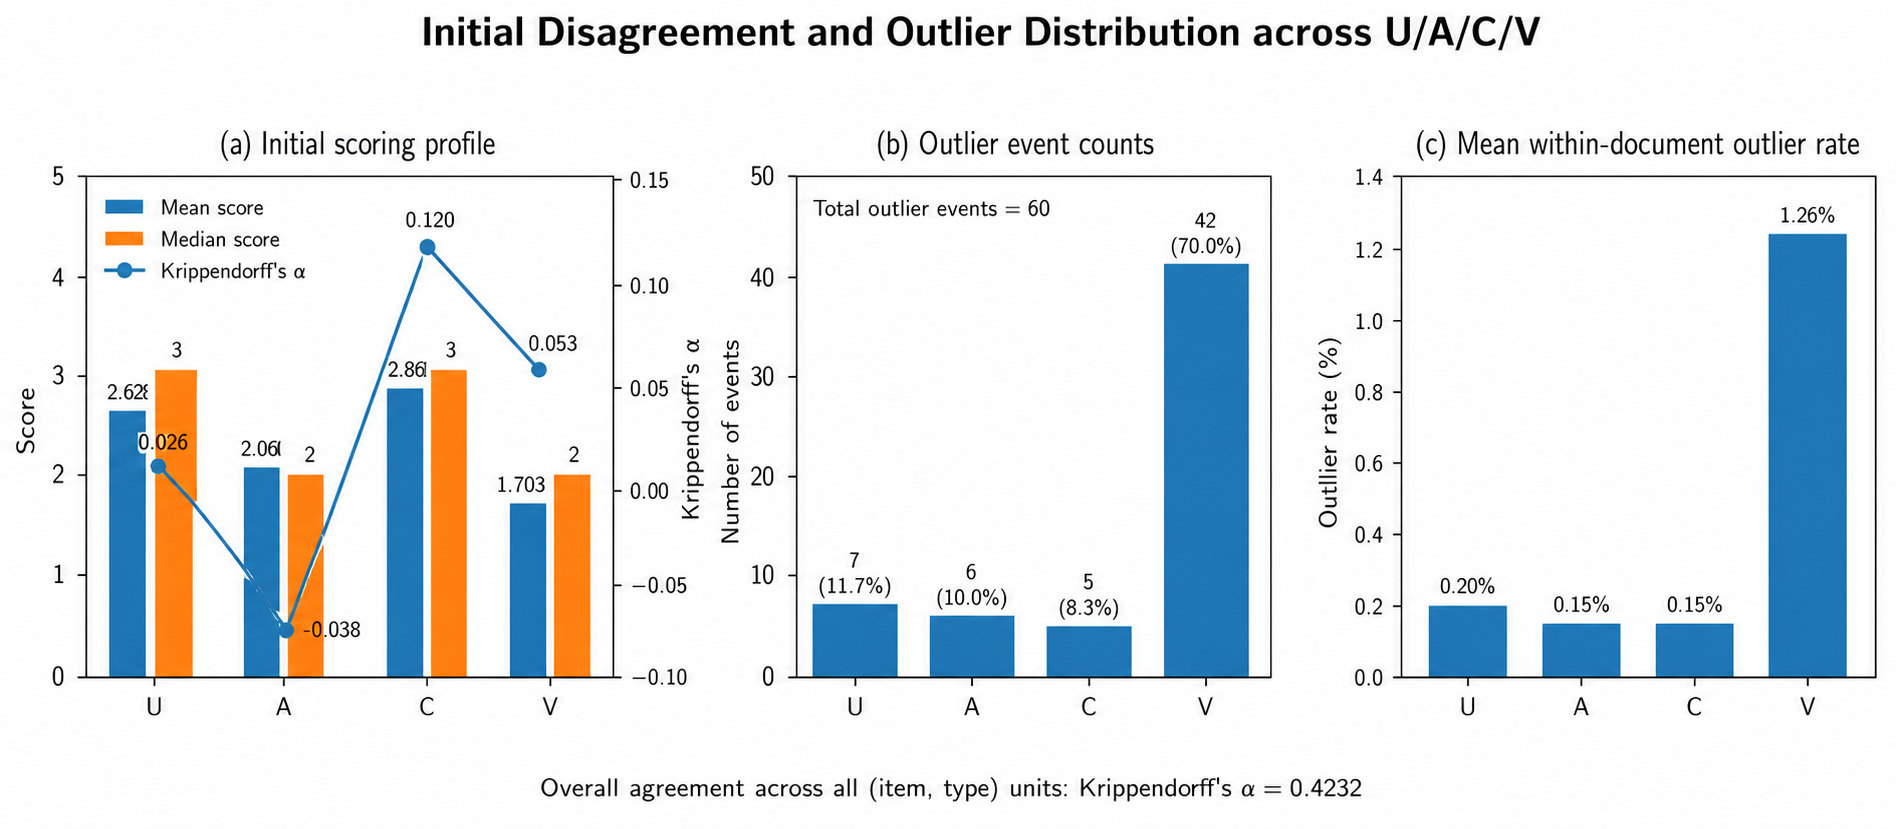
\includegraphics[width=\linewidth]{figures/fig2_rq1_disagreement.png}
\caption{Initial disagreement and outlier distribution across U/A/C/V.}
\label{fig:rq1_disagreement}
\end{figure}

\subsection{RQ2：How does the proposed workflow compare with individual LLMs and aggregation baselines?}
RQ2 评估本文提出的 outlier-aware consensus workflow 在生成逐条需求问题清单时，相较于单模型、等权聚合和无权重圆桌基线的表现与权衡。为避免将整体性能变化直接归因于某一个组件，本节依次报告离群质量判别、treatment-level Ground Truth 对齐性能、模型画像与固定权重消融，以及圆桌收敛和问题清单规模。

\subsubsection{Good and Bad Outlier Separation}
对 60 个离群事件进行论证质量评分与决策后，当前规则下共有 26 个事件被判定为 \texttt{good}，15 个被判定为 \texttt{bad}，19 个被判定为 \texttt{uncertain}。整体 hard-fail 率为 $21.67\%$，且触发 hard-fail 的事件最终 $100.00\%$ 被归入 \texttt{bad}，证明该底线规则有效拦截了低质量偏离。综合论证质量分在三类离群之间呈现出清晰分层：\texttt{good} 事件的中位数为 $0.7500$，均值为 $0.7788$；\texttt{bad} 事件的中位数为 $0.2500$，均值为 $0.3056$；\texttt{uncertain} 事件介于二者之间，中位数为 $0.4167$，均值为 $0.4386$。Mann--Whitney U 检验显示，\texttt{good} 与 \texttt{bad} 的分布差异显著（$p<0.05$）；将 \texttt{bad} 与 \texttt{uncertain} 合并为 \texttt{non-good} 后，\texttt{good} 与 \texttt{non-good} 之间的差异同样显著（$p<0.05$）。由此可见，当前离群判别机制并非只依赖“偏离幅度大”的单一信号，而是能够结合文本证据深度，实现高价值异议与低质量偏离的有效分离。

\begin{table*}[t]
\centering
\caption{Representative good and bad outlier cases.}
\label{tab:representative_outlier_cases}
\renewcommand{\arraystretch}{1.15}
\resizebox{\textwidth}{!}{%
\begin{tabular}{p{1.0cm}p{1.6cm}p{0.8cm}p{1.4cm}p{1.2cm}p{2.8cm}p{3.1cm}p{3.2cm}}
\toprule
\textbf{Case} &
\textbf{Item} &
\textbf{Type} &
\textbf{Score / Median} &
\textbf{Decision} &
\textbf{Requirement excerpt} &
\textbf{Model evidence} &
\textbf{Adjudication rationale} \\
\midrule

G1 &
\texttt{[doc--item]} &
V &
\texttt{[score]/[median]} &
Good &
\textit{``[short requirement excerpt]''} &
\textit{``[evidence span or model explanation]''} &
The outlier is retained because the model identifies a concrete verifiability problem, provides a traceable textual cue, and proposes a testable or measurable revision. \\

\midrule

G2 &
\texttt{[doc--item]} &
A &
\texttt{[score]/[median]} &
Good &
\textit{``[short requirement excerpt]''} &
\textit{``[evidence span or model explanation]''} &
The outlier is retained because the minority judgment exposes an ambiguity that is not captured by the group median, while the evidence and rewrite suggestion remain dimension-aligned and actionable. \\

\midrule

B1 &
\texttt{[doc--item]} &
U &
\texttt{[score]/[median]} &
Bad &
\textit{``[short requirement excerpt]''} &
\textit{``[evidence span or model explanation]''} &
The outlier is rejected because the explanation is weak or generic, does not clearly identify a textual defect, and therefore fails to justify the large deviation from the group median. \\

\midrule

B2 &
\texttt{[doc--item]} &
C &
\texttt{[score]/[median]} &
Bad &
\textit{``[short requirement excerpt]''} &
\textit{``[evidence span or model explanation]''} &
The outlier is rejected because it reflects a dimension mismatch or an unsupported correctness claim rather than a demonstrable defect in the requirement statement. \\

\bottomrule
\end{tabular}%
}

\vspace{0.4em}
\begin{minipage}{0.97\textwidth}
\footnotesize
\textit{Note.}
Good outliers are minority judgments that deviate from the group median but provide sufficient evidence, dimension-aligned reasoning, and executable rewrite suggestions. Bad outliers are deviations rejected by the argument-quality assessment or hard-fail rules, such as missing evidence, non-executable rewrite suggestions, or dimension mismatch. Placeholders in square brackets should be replaced with real representative cases; the complete cases are provided in the replication package.
\end{minipage}
\end{table*}


\begin{figure}[t]
\centering
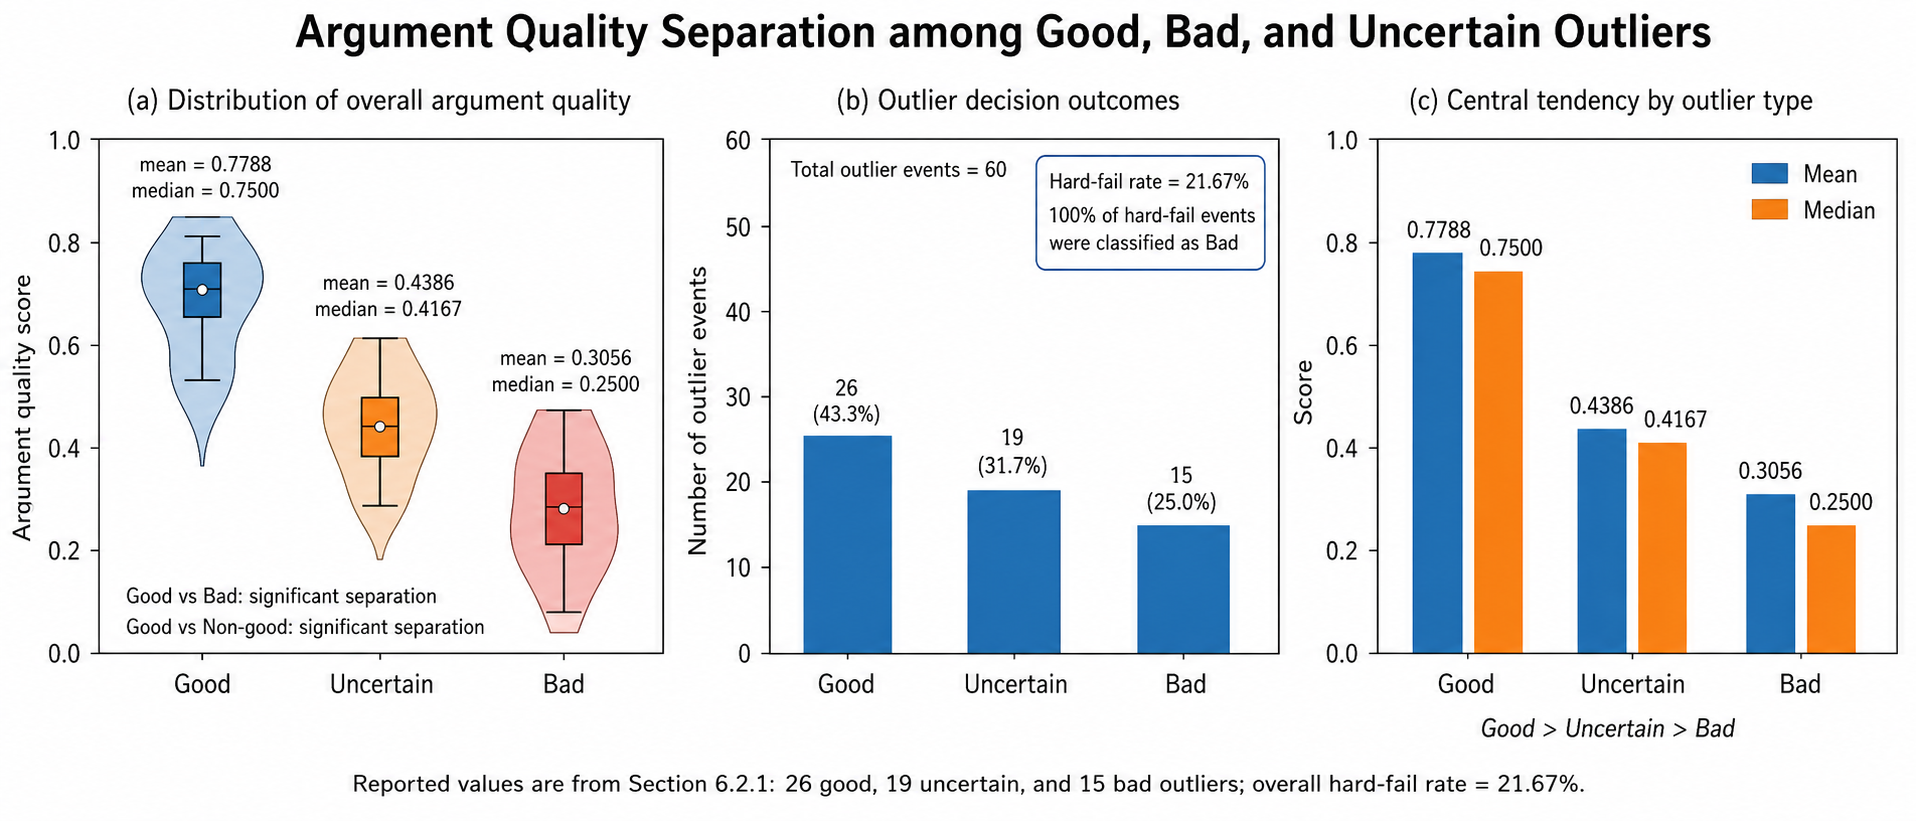
\includegraphics[width=\linewidth]{figures/fig3_outlier_separation.png}
\caption{Argument-quality separation among good, bad, and uncertain outliers.}
\label{fig:outlier_separation}
\end{figure}

\subsubsection{Treatment-level Performance}
\begin{table*}[t]
\centering
\caption{Treatment-level performance results.}
\label{tab:treatment_results}
\renewcommand{\arraystretch}{1.15}
\resizebox{\textwidth}{!}{%
\begin{tabular}{p{2.8cm}cccp{1.6cm}p{3.4cm}p{2.4cm}}
\toprule
\textbf{Treatment} &
\textbf{Macro-P} &
\textbf{Macro-R} &
\textbf{Macro-F1} &
\textbf{Avg.\ pred.\ issues} &
\textbf{Primary characteristic} &
\textbf{Role} \\
\midrule

Single-LLM Family Mean
& 0.0769
& ---
& 0.0960
& ---
& Balanced single-model behaviour
& Reference \\

Equal-Weight Aggregation
& 0.0771
& 0.4077
& \textbf{0.1153}
& 144.8
& Highest recall; very large issue list
& Aggregation baseline \\

Roundtable No Weighting
& ---
& ---
& 0.0968
& 136.7
& Consensus without reliability-aware weighting
& Ablation \\

Full Method
& \textbf{0.0901}
& 0.1354
& 0.0711
& \textbf{15.9}
& Highest precision; strongest issue-list compression
& Proposed \\

\bottomrule
\end{tabular}%
}

\vspace{0.4em}
\begin{minipage}{0.97\textwidth}
\footnotesize
\textit{Overall comparison.} Friedman test on document-level Macro-F1 finds no statistically significant overall difference among the four treatments ($p>0.05$). Although the proposed Full Method does not achieve the highest Macro-F1, it produces substantially more compact issue lists while improving precision, indicating a selective issue-generation strategy rather than a high-recall detector.
\textit{Note.} Macro-P = Macro-Precision; Macro-R = Macro-Recall. All performance values are averaged over the 10 shared requirements documents. Cells marked ``---'' denote values not emphasized in the current paper and can be added if desired.
\end{minipage}
\end{table*}

在 10 份共同文档的严格配对比较中，四类方法的文档级 Macro-F1 均值呈现出一定差异：Equal-Weight Aggregation 的平均值最高（$0.1153$），其次为 Roundtable No Weighting（$0.0968$）与 Single-LLM Family Mean（$0.0960$），而 Full Method 的平均值最低（$0.0711$）。然而，Friedman 检验未发现四类方法之间存在统计显著的总体差异（% TODO: 从 main.docx 补全 $\chi^2$、$p$、Kendall's $W$
$p>0.05$），表明方法间差异的效应量较小。因此，该结果不能支持某一方法在文档级 Macro-F1 上具有稳定优势。

我们认为可能的原因是，Full Method 的设计目标并非最大化平均分数或简单提高标签重合率，而是通过离群识别、模型画像和动态置信度机制生成更可审查的问题清单。从 Precision 和 Recall 的组合来看，Full Method 表现出明显的选择性输出倾向：其 Macro-Precision 为 $0.0901$，高于 Equal-Weight 的 $0.0771$ 和 Single-LLM Family Mean 的 $0.0769$；然而其 Macro-Recall 仅为 $0.1354$，显著低于 Equal-Weight 的 $0.4077$。结合平均预测问题量可以进一步解释这一现象：Full Method 平均每份文档仅输出 $15.9$ 个问题，而 Equal-Weight 平均输出 $144.8$ 个问题。因此，Full Method 并不是一个高召回的问题发现器，而是一个更精简、相对更高 Precision、更选择性的问题清单生成流程。

\subsubsection{Model Profiling and Fixed Weighting (Ablation)}
为了探究固定模型权重的实际效用，我们对模型画像进行了分析。5 个模型的平均固定权重分别为：DeepSeek（$0.3129$）、GPT（$0.2738$）、Kimi（$0.2732$）、Qwen（$0.2598$）和 GLM-5（$0.1437$）。值得注意的是，平均固定权重与单模型的平均 Macro-Recall / Macro-F1 均呈强负相关（分别为 $-0.8000$ 和 $-0.9000$）。这印证了本文的假设：固定权重不是模型综合分类能力的静态排序，而是对其在当前文档内捕捉“高价值离群”贡献的动态度量。同时，我们设定的 \texttt{full\_method\_equal\_weights} 消融实验（用等权重替换模型画像权重）进一步量化了该模块的贡献：Full Method（$0.0711$）与等权重版本（$0.0704$）的 Macro-F1 几乎一致（Wilcoxon 配对检验 $p=0.7500$），区别仅在于引入画像权重后最终预测问题数从 $17.6$ 进一步微降至 $15.9$。这提示我们，本文方法的主要可观察效果来自离群感知过滤、问题集合收敛与最终清单压缩的组合，而不是直接提升宏观分类指标。

\subsubsection{Roundtable Convergence and Issue-list Compactness}
圆桌共识表现出极强的集合层面收敛性。我们以 Full Method 与 Roundtable No Weighting 作为主要对比单元：10 份共同文档中，Full Method 的问题收敛成功率（\texttt{issue\_converged}）高达 $100.00\%$，最终轮次平均 issue-set Jaccard 相似度达 $0.9838$，平均最终的最大评分分差（\texttt{max\_score\_diff}）为 $0.7819$。相比之下，Roundtable No Weighting 的问题收敛成功率为 $90.00\%$，最终轮平均 issue-set Jaccard 为 $90.02\%$，平均最终的最大评分分差为 $1.1789$。而所有方法的评分收敛率均为 $0.00\%$，说明问题集合趋同并不等同于评分完全收敛，而是问题集合的统一先于数值评分的一致。从问题清单规模看，Full Method 在 10 份共同文档范围内将 611 个初始候选问题大幅压缩至 159 个最终问题，整体保留率仅为 $26.02\%$；在同一口径下，Full Method 的平均预测问题数为 $15.9$，Roundtable No Weighting 为 $136.7$，Equal-Weight Aggregation 为 $144.8$。该结果表明，outlier-aware consensus workflow 能够大幅减少最终输出的问题数量，并形成更稳定的问题集合，极大提升了最终输出的紧凑性和工程可操作性。

\begin{figure}[t]
\centering
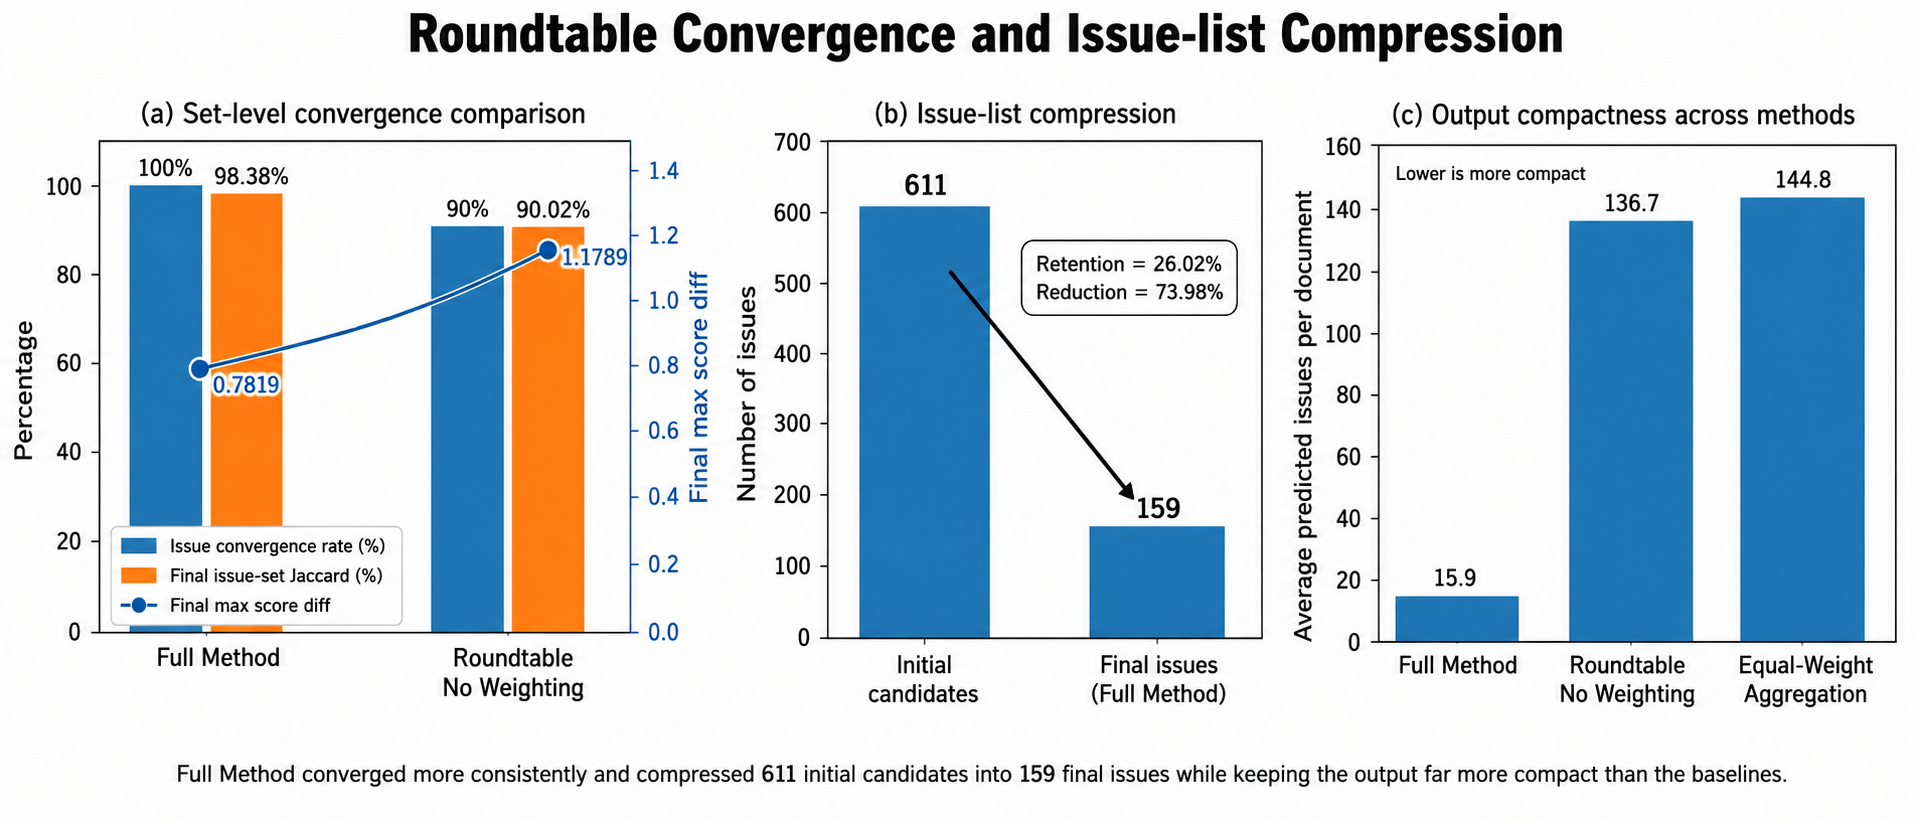
\includegraphics[width=\linewidth]{figures/fig4_convergence.png}
\caption{Roundtable convergence and issue-list compression.}
\label{fig:convergence}
\end{figure}

\textit{Result for RQ2:} 本文工作流并非在所有传统性能指标上单向超越基线，而是体现为一种清晰的权衡。它能有效识别异议质量，生成集合高度稳定、紧凑且精确率更高的问题清单；但这以牺牲召回率为代价。消融实验证明，画像定权机制的边际效用在于强化候选问题压缩，而非提升 F1 指标。

\subsection{RQ3：How does the workflow vary across documents and quality dimensions?}
实验结果显示，Full Method 的表现具有明显的文档异质性与维度倾向。\textbf{文档层面}：在初始候选问题密集的文档上，该框架带来了可观的 F1 提升。例如 \texttt{2005 - phin}（初始问题 200 个被压缩至 10 个），Macro-F1 从 $0.0859$ 跃升至 $0.1667$；\texttt{2007 - puget sound} 的 Macro-F1 从 $0.1498$ 升至 $0.1867$。然而，这些增益主要源于冗余过滤带来的 Precision 改善，同时不可避免地伴随了 Recall 的下降。\textbf{维度层面}：以去重后的 $(item,type)$ 候选计算，初始候选问题清单中 U/A/C/V 分布较为均衡（占比分别约 $25\%$、$26\%$、$20\%$、$29\%$），但经过全流程后，最终问题清单中 U/A/C/V 占比剧变为 $1.26\%$、$39.62\%$、$0.00\%$、$59.12\%$。系统极度倾向于保留可验证性（V）与无歧义性（A）问题。

\begin{figure}[t]
\centering
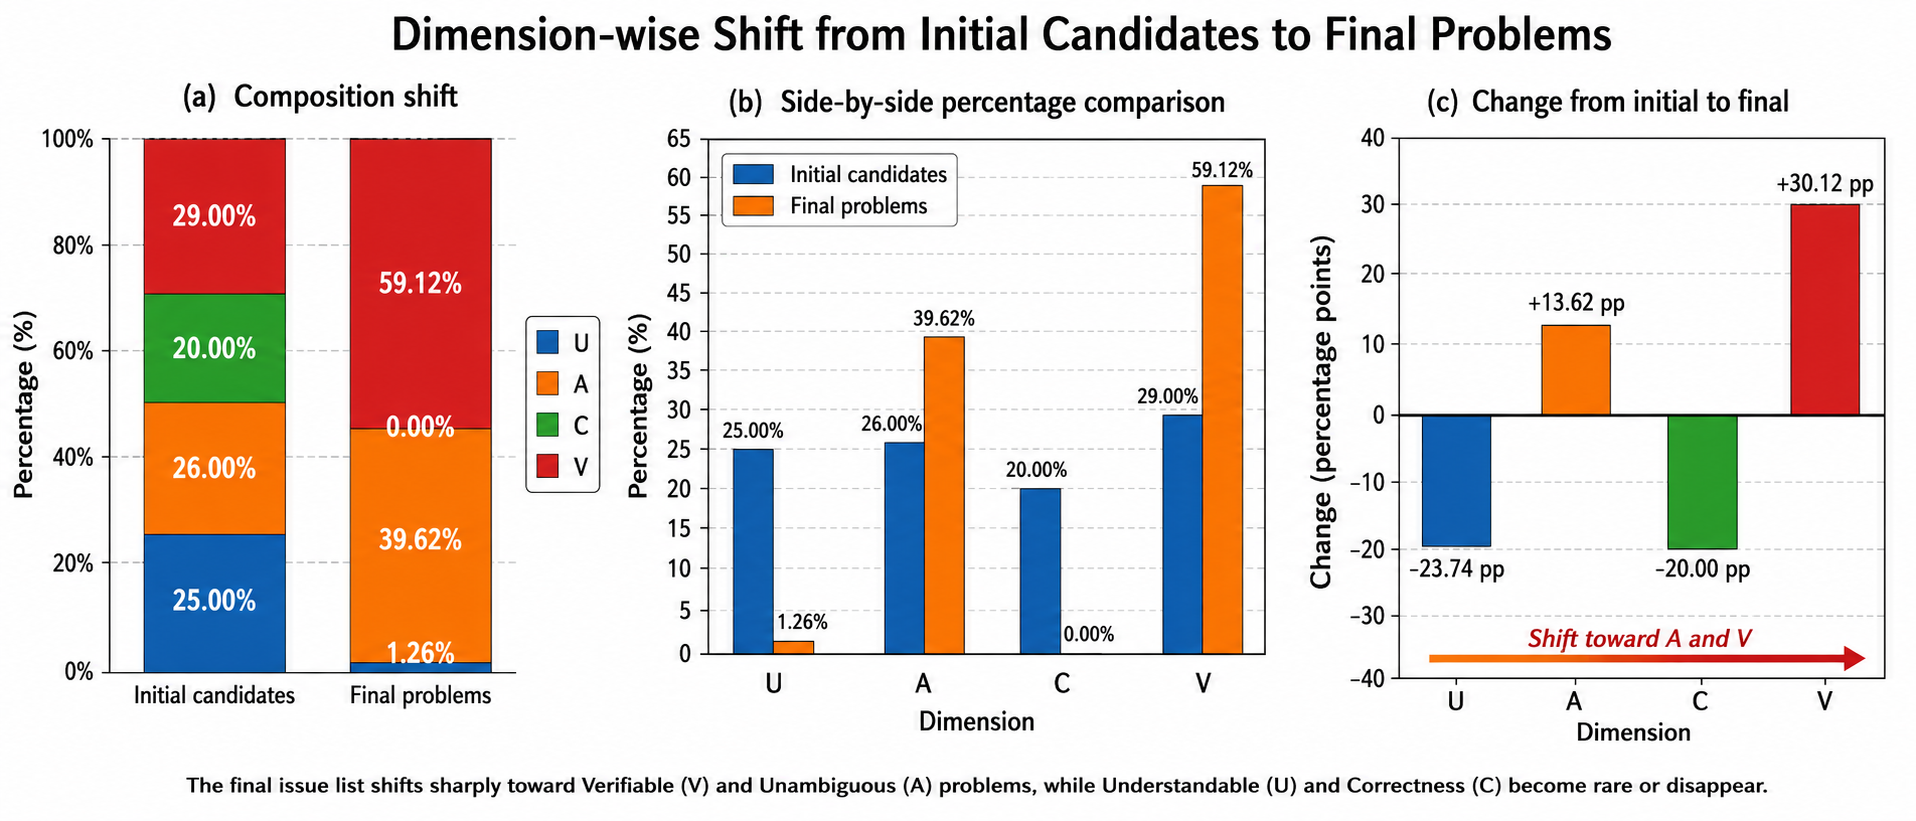
\includegraphics[width=\linewidth]{figures/fig5_dimension_shift.png}
\caption{Dimension-wise shift from initial candidates to final problems.}
\label{fig:dimension_shift}
\end{figure}

\textit{Result for RQ3:} outlier-aware consensus workflow 的表现高度依赖上下文。在候选问题密集的文档中，其精简效应最能转化为精确率增益。同时，最终输出高度聚焦于 V 和 A 类缺陷，这反映了模型交互在此类形式化/语义界限明确的任务上更易达成理性共识。

\subsection{Summary of Findings}
综合上述实证分析，本文得出以下四个核心结论：（1）\textbf{结构性分歧存在}：不同 LLM 在逐条需求质量识别中并非产生随机噪声，而是在 V 维度上表现出显著的结构性离群集中度；（2）\textbf{权衡型性能图景}：outlier-aware consensus workflow 能精准分离好坏离群，生成规模紧凑、精确率更高、集合高度稳定的专家级问题清单，但无法在统计上避免明显的召回率折损；（3）\textbf{定权机制的定界}：通过模型画像进行的固定权重分配，其核心功能在于进一步平滑并压缩冗余候选，而非创造显著的 Macro-F1 增益；（4）\textbf{泛化异质性}：框架优势主要集中于候选问题密集型文档的去噪，且最终输出强烈偏向可验证性（V）与无歧义性（A）维度。

\section{Validity Threats and Discussion}
\label{sec:validity}
\subsection{Validity Threats}
\subsubsection{Construct Validity}
建构效度主要涉及理论概念与实际度量指标之间的匹配程度。本研究的核心威胁在于论证质量（$Q$）分数的计算公式、六维特征的定义以及硬性否决（Hard Fail）机制的设定，这些规则与经验阈值可能存在一定的主观偏置。\textit{Mitigation:} 本文的维度定义（U/A/C/V）严格映射自经典的 IEEE 需求规格说明标准与已有的实证软件工程分类法；对于 $Q$ 分数的量化，我们避免了复杂的非线性赋权，而是采用简单的均匀归一化并辅以底线阻断（Hard Fail），以剥离过度拟合的风险。消融对比（无定权圆桌与完整方法）已侧面证明当前参数设置足以在实际任务中产生显著区分度。

\subsubsection{Internal Validity}
内部效度关注实验执行中可能干扰因果关系的实现细节。核心威胁来自真实 API 服务的不稳定性：限流、超时或非法的 JSON 输出会导致部分模型在特定条目上被跳过，这意味着不同文档或条目上的实际有效模型数并不完全一致。其次，当前实验参数（离群阈值、好/坏离群阈值、惩罚系数、Top-K 和最大轮次等）均基于经验设置。\textit{Mitigation:} 我们将 API 不稳定性显式纳入系统的稳健性考量：系统部署了重试与 case 级隔离机制，当某模型彻底失败时仅在该需求条目上禁用该模型，其余模型继续完成圆桌；实验结果以文档级 Macro-F1 汇总，有效稀释了单一条目请求丢失带来的随机影响。

\subsubsection{External Validity}
外部效度涉及研究结论向其他场景或未来模型泛化的能力。首先，PURE 数据集虽然真实，但主要代表传统的系统规格说明书（SRS），可能无法直接推演至高度敏捷开发中的用户故事或特定合规领域；其次，实验选定的 5 款异构 LLM 具有时效性。\textit{Mitigation:} 在文档选择上，我们抽取了覆盖不同领域、规模与缺陷密度的样本；在模型层面，本研究验证的是“基于价值判别的动态定权与圆桌框架”这一方法论的可行性，而非对当前几款模型的永久性排序，该框架在理论上与底层具体模型解耦。

\subsubsection{Conclusion Validity}
结论效度关注统计分析是否足以支撑研究推论。主要威胁在于文档间异质性带来的统计偏差，若直接将所有需求条目混合计算 $p$ 值，极易引发辛普森悖论。\textit{Mitigation:} 在统计设计上，我们严格采用“Document”作为配对比较的 Block 单元，使用鲁棒的非参数统计方法（Friedman 检验与配对 Wilcoxon 符号秩检验）并强制报告非参数效应量（Cliff's $\delta$），以规避分布异质性带来的误判。

\subsection{Discussion}
综合上述结果与威胁分析，本文当前最重要的启示有三点。第一，在多 LLM 需求审查中，“少数派意见”不是应被直接抹平的噪声，而是应被进一步审查的潜在信息源；关键不在于是否偏离共识，而在于偏离是否具备高质量证据与可执行改写。第二，模型定权不应被理解为对模型能力的静态排序，而应被理解为一种文档内、任务内的证据驱动型信任分配机制。第三，圆桌共识的主要价值不是让模型的数值评分完全一致，而是帮助系统在有限轮次内稳定形成更紧凑、更可操作的问题集合。总体上，当前结果支持本文方法作为一种“从分歧到共识”的需求质量审查框架具有可行性，但仍需在更大规模对照实验中进一步验证。

\section{Conclusion}
\label{sec:conclusion}
多大语言模型（LLM）在软件工程任务中的集成应用，长期受制于“趋同即正确”的多数表决假设，导致高价值的少数派意见极易被群体的平滑效应所抹杀。针对这一“共识谬误”，本研究构建了一种面向逐条需求（per-requirement）质量评估的异构多模型圆桌共识框架。通过引入基于文本论证深度的离群判别机制，本框架建立了一套将模型间的“结构化分歧”转化为全局信任权重的量化方法，并在多轮交互中融合该静态权重与动态置信度，驱动评审团队达成理性共识。

实证结果确立了需求质量自动化审查领域的一个关键认知转移：在复杂的工程推演任务中，评分分歧本身即是极具鉴别力的度量信号。本研究证明，依靠证据充分性与改写可执行性等特征构成的论证质量向量，系统能够有效穿透数值层面的偏差，精准阻断缺乏依据的幻觉（坏离群），同时系统性地放大具备深层逻辑发现能力的少数派意见（好离群）。相较于传统的等权集成方法，基于离群历史画像的定权与圆桌机制能够在有限轮次内实现缺陷集合的快速收敛。基于当前发现，未来工作可沿三个方向展开：将该多代理审查框架推广至敏捷 User Stories 乃至系统架构设计文档；在论证质量向量中显式引入跨条目一致性检验与外部领域知识约束；以及探索在极端异质化或端侧部署环境下更细粒度的本地容错与模型替补策略。

\begin{thebibliography}{99}
\bibitem{ref1} Requirements Engineering Artifact Quality: Definition and Control.
\bibitem{ref2} Empirical research on requirements quality: a systematic mapping study.
\bibitem{ref3} Requirements quality research: a harmonized theory, evaluation, and roadmap.
\bibitem{ref4} Requirements Quality Is Quality in Use.
\bibitem{ref5} Rapid Quality Assurance with Requirements Smells.
\bibitem{ref6} Improving agile requirements: the Quality User Story framework and tool.
\bibitem{ref7} Improving Requirements Quality using Essential Use Case Interaction Patterns.
\bibitem{ref8} Poster: Analysis of Requirements Quality Evolution.
\bibitem{ref9} PURE: a Dataset of Public Requirements Documents.
\bibitem{ref10} Using LLMs in Software Requirements Specifications: An Empirical Evaluation.
\bibitem{ref11} Large Language Models (LLMs) for Requirements Engineering (RE): A Systematic Literature Review.
\bibitem{ref12} Multi-Agent Debate Strategies to Enhance Requirements Engineering with Large Language Models.
\bibitem{ref13} Can LLMs Replace Human Evaluators? An Empirical Study of LLM-as-a-Judge in Software Engineering.
\bibitem{ref14} Are Large Language Models Reliable Judges? A Study on the Factuality Evaluation Capabilities of LLMs.
\bibitem{ref15} Improving Factuality and Reasoning in Language Models through Multiagent Debate.
\bibitem{ref16} Encouraging Divergent Thinking in Large Language Models through Multi-Agent Debate.
\bibitem{ref17} METAGPT: Meta Programming for a Multi-Agent Collaborative Framework.
\bibitem{ref18} RECONCILE: Round-Table Conference Improves Reasoning via Consensus among Diverse LLMs.
\bibitem{ref19} Voting or Consensus? Decision-Making in Multi-Agent Debate.
\bibitem{ref20} Exchange-of-Thought: Enhancing Large Language Model Capabilities through Cross-Model Communication.
\bibitem{ref21} Maximum Likelihood Estimation of Observer Error Rates Using the EM Algorithm.
\bibitem{ref22} Whose Vote Should Count More: Optimal Integration of Labels from Labelers of Unknown Expertise.
\bibitem{ref23} Truth Is a Lie: Crowd Truth and the Seven Myths of Human Annotation.
\bibitem{ref24} Learning Whom to Trust with MACE.
\bibitem{ref25} Learning from Disagreement: A Survey.
\bibitem{ref26} Wisdom of Instruction-Tuned Language Model Crowds: Exploring Model Label Variation.
\end{thebibliography}

\end{document}
